\textbf{Ejercicio 27:} Calcular el volumen de la región limitada por $x^2 + y^2 = 2ax$, $x^2 + y^2 = az$ y $z = 0$ con $a \in \mathbb{R} \setminus \{0\}$.

Para calcular el volumen de una región sólida $W$, partimos de la definición 2.5.6:

\begin{equation}
    V = \iiint_{W} 1 \, dV
\end{equation}

Previo a integrar, resulta conveniente identificar las distintas superficies que conforman la frontera de $W$, teniendo en cuenta que las mismas dependen del parametro $a$:
\begin{itemize}
    \item \textbf{Cilindro:} $x^2 + y^2 = 2ax \implies (x-a)^2 + y^2 = a^2$. Es un cilindro circular de radio $|a|$ con centro en $(a,0)$.
    \item \textbf{Paraboloide:} $z = \frac{x^2 + y^2}{a}$. Es la superficie que limita la altura del sólido. Para valores de $a > 0$ el paraboloide es el techo de la superficie mientras que para valores de $a < 0$ es el piso de la superficie. 
    \item \textbf{Plano $xy$:} $z = 0$.
\end{itemize}


\begin{figure}[htbp]
    \centering
    % ESTA LÍNEA es la que crea el PDF en la carpeta /tikz
    \tikzsetnextfilename{ejercicio27_figura} 
    
    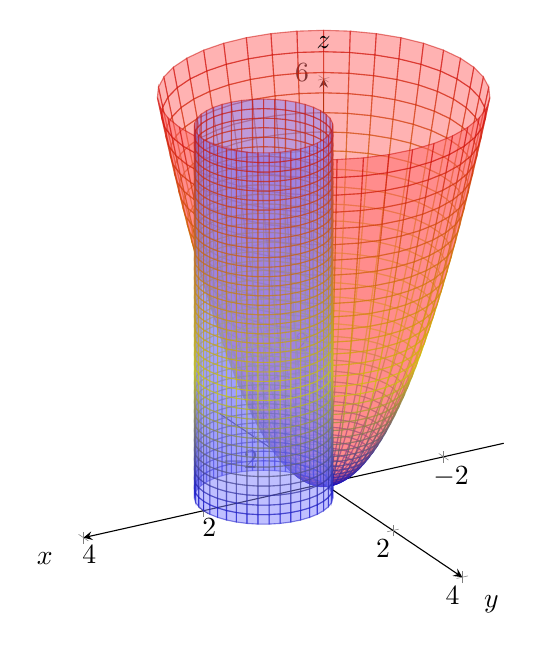
\begin{tikzpicture}
        \begin{axis}[
            view={150}{25}, % Cámara: eje x hacia adelante/izq, eje y hacia la derecha
            width=10cm,
            height=10cm,
            grid=major,
            xmin=-3, xmax=4, % Ajusté un poco los ejes para que se vea mejor
            ymin=-3, ymax=4,
            zmin=0, zmax=6,
            axis lines=center,
            xlabel={$x$},
            ylabel={$y$},
            zlabel={$z$},
            % Estos 3 comandos evitan que las letras queden flotando en cualquier lado
            every axis x label/.style={at={(ticklabel* cs:1.05)},anchor=north east},
            every axis y label/.style={at={(ticklabel* cs:1.05)},anchor=north west},
            every axis z label/.style={at={(ticklabel* cs:1.05)},anchor=south},
        ]

        % Paraboloide z = x^2 + y^2 (Rojo)
        \addplot3[
            surf,
            domain=0:360,
            y domain=0:2.4,
            samples=40,
            color=red!60,
            opacity=0.5,
            z buffer=sort, % Esto arregla el renderizado de la transparencia
        ]
        ({y*cos(x)}, {y*sin(x)}, {y^2});

        % Cilindro (x-1)^2 + y^2 = 1 (Azul)
        \addplot3[
            surf,
            domain=0:360,
            y domain=0:5.5,
            samples=40,
            color=blue!50,
            opacity=0.5,
            z buffer=sort, % Esto arregla el renderizado de la transparencia
        ]
        ({1+cos(x)}, {sin(x)}, {y});

        \end{axis}
    \end{tikzpicture}
    \caption{Representación de la región $W$. \href{https://www.geogebra.org/classic/q6ujp7ap}{Ver en GeoGebra}}
\end{figure}
     
Para resolver la integral, se usará el Teorema 2.5.2. Se usara el cambio de variable famoso, conocido como coordenadas cilindricas. Entonces, la transformacion resulta ser:

\begin{equation*}
    \begin{cases} 
        x = r \cos \theta \\ 
        y = r \sin \theta \\ 
        z = z 
    \end{cases}
\end{equation*}

La región transformada $W^*$ depende del signo del parámetro $a$, ya que el cilindro $r = 2a\cos\theta$ debe representar radios positivos.

\begin{itemize}

\item \textbf{Si $a>0$:}

\begin{equation*}
W^*:
\begin{cases}
-\frac{\pi}{2} \le \theta \le \frac{\pi}{2} \\
0 \le r \le 2a \cos \theta \\
0 \le z \le \frac{r^2}{a}
\end{cases}
\end{equation*}

\item \textbf{Si $a<0$:}

Para que $r \le 2a\cos\theta$ sea positivo, debe cumplirse $\cos\theta <0$, por lo que:

\begin{equation*}
W^*:
\begin{cases}
\frac{\pi}{2} \le \theta \le \frac{3\pi}{2} \\
0 \le r \le 2a \cos \theta \\
\frac{r^2}{a} \le z \le 0
\end{cases}
\end{equation*}

\end{itemize}

Una vez ya definidos los limites de integracion, usando el teorema de cambio de variable para integrales triples resulta que:

\begin{align}
V &= \iiint_{W} 1 \, dV \\
V &= \iiint_{W^*} |J_{\mathbf{T}}| \, dz \, dr \, d\theta \\
V &= \iiint_{W^*} r\, dz \, dr \, d\theta
\end{align}

\begin{itemize}

\item 

Caso 1: $a > 0$

En este caso, el sólido está por encima del plano $xy$ ($0 \le z \le \frac{r^2}{a}$) y el cilindro se encuentra en el semiplano $x > 0$, por lo que $\theta \in [-\frac{\pi}{2}, \frac{\pi}{2}]$.

\begin{align*}
V &= \int_{-\frac{\pi}{2}}^{\frac{\pi}{2}} \int_{0}^{2a \cos \theta} \int_{0}^{\frac{r^2}{a}} r \, dz \, dr \, d\theta \\
V &= \int_{-\frac{\pi}{2}}^{\frac{\pi}{2}} \int_{0}^{2a \cos \theta} \frac{r^3}{a} \, dr \, d\theta \\
V &= \frac{1}{a} \int_{-\frac{\pi}{2}}^{\frac{\pi}{2}} \left[ \frac{r^4}{4} \right]_{0}^{2a \cos \theta} \, d\theta \\
V &= \frac{1}{4a} \int_{-\frac{\pi}{2}}^{\frac{\pi}{2}} 16a^4 \cos^4 \theta \, d\theta \\
V &= 4a^3 \int_{-\frac{\pi}{2}}^{\frac{\pi}{2}} \cos^4 \theta \, d\theta
\end{align*}

Utilizando la identidad $\cos^4 \theta = (\frac{1+\cos(2\theta)}{2})^2 = \frac{1}{4}(1 + 2\cos(2\theta) + \cos^2(2\theta))$ y luego $\cos^2(2\theta) = \frac{1+\cos(4\theta)}{2}$:

\begin{align*}
V &= 4a^3 \int_{-\frac{\pi}{2}}^{\frac{\pi}{2}} \left( \frac{3}{8} + \frac{1}{2}\cos(2\theta) + \frac{1}{8}\cos(4\theta) \right) \, d\theta \\
V &= 4a^3 \left[ \frac{3}{8}\theta + \frac{1}{4}\sin(2\theta) + \frac{1}{32}\sin(4\theta) \right]_{-\frac{\pi}{2}}^{\frac{\pi}{2}} \\
V &= 4a^3 \left( \frac{3\pi}{8} \right) \\
V &= \frac{3}{2}\pi a^3
\end{align*}

\item 

Caso 2: $a < 0$

En este caso el paraboloide abre hacia abajo, por lo que $\frac{r^2}{a} \le z \le 0$, y el cilindro se encuentra en el semiplano $x < 0$, lo que implica $\theta \in [\frac{\pi}{2}, \frac{3\pi}{2}]$.

\begin{align*}
V &= \int_{\frac{\pi}{2}}^{\frac{3\pi}{2}} \int_{0}^{2a \cos \theta} \int_{\frac{r^2}{a}}^{0} r \, dz \, dr \, d\theta \\
V &= \int_{\frac{\pi}{2}}^{\frac{3\pi}{2}} \int_{0}^{2a \cos \theta} r \left(0 - \frac{r^2}{a}\right) dr \, d\theta \\
V &= \int_{\frac{\pi}{2}}^{\frac{3\pi}{2}} \int_{0}^{2a \cos \theta} -\frac{r^3}{a} \, dr \, d\theta \\
V &= -\frac{1}{a} \int_{\frac{\pi}{2}}^{\frac{3\pi}{2}} \left[ \frac{r^4}{4} \right]_{0}^{2a \cos \theta} d\theta \\
V &= -\frac{1}{4a} \int_{\frac{\pi}{2}}^{\frac{3\pi}{2}} 16a^4 \cos^4 \theta \, d\theta \\
V &= -4a^3 \int_{\frac{\pi}{2}}^{\frac{3\pi}{2}} \cos^4 \theta \, d\theta
\end{align*}

Como $\cos^4\theta$ es periódica y par respecto a $\pi$, se tiene

\[
\int_{\frac{\pi}{2}}^{\frac{3\pi}{2}} \cos^4\theta \, d\theta =
\int_{-\frac{\pi}{2}}^{\frac{\pi}{2}} \cos^4\theta \, d\theta
\]

por lo que

\begin{align*}
V &= -4a^3 \left(\frac{3\pi}{8}\right) \\
V &= -\frac{3}{2}\pi a^3
\end{align*}

Como $a<0$, entonces $a^3<0$, y por lo tanto el volumen resulta positivo.

\end{itemize}

Combinando ambos casos, el volumen del sólido para cualquier $a \neq 0$ es:

\begin{equation}
V = \frac{3}{2}\pi |a|^3
\end{equation}
